
\documentclass{article}
    \usepackage[utf8]{inputenc}
    \usepackage{comment}
    \usepackage{environ}
    \usepackage{listings}
    \usepackage{xcolor}
    \usepackage[letterpaper, portrait, margin=1in]{geometry}
    \usepackage{amsmath}
    \usepackage{amssymb}
    \usepackage{graphicx}
    \usepackage{hyperref}
    
    \newif\ifshowsolutions
    
    % comment the following line to hide solutions
    \showsolutionstrue
    
    \ifshowsolutions
        \newenvironment{solution}{

            \color{blue} \smallskip \textbf{Solution:}}{}
    \else
        \NewEnviron{solution} {
            \ \\
            \ \\
            \ \\
            \ \\
            \ \\
        }
    \fi
    
    \begin{document}
    
    \part*{Continuous and Joint Distributions Practice}
    \vspace{-7pt}
    \hrule
    \vspace{7pt}
    I chose to pick a lot of midterm and final problems for practice this week. Some of these are quite challenging, but interesting!
    \begin{enumerate}
        \item (Spring 2017, 5.9) What is the probability density function for a continuous random variable with $Pr(X \leq x) = 1 - \frac{1}{x}$ for $x \geq 1$ and $Pr(X \leq x) = 0$ for $x < 1$?
        \begin{solution}
            We are basically given the CDF, defined as $F_X(x) = P(X \leq x)$, and we want to find the PDF, which is $f_X(x) = \frac{d F_X(x)}{dx}$. Then \[
                f_X(x) = \left(1 - \frac{1}{x}\right)' = \frac{1}{x^2}
            \]
            That is for $x \geq 1$. When $x < 1$, because the CDF is 0, its derivative is also 0. Then \[
                f_X(x) = \begin{cases}
                    \frac{1}{x^2} & \text{if } x \geq 1 \\
                    0 & \text{otherwise}
                \end{cases}
            \]
        \end{solution}
        \item (Fall 2017, 6.10) $X$ and $Y$ are continuous random variables and are uniformly distributed with pdf $f(x, y) = c$ over their
        region of support (the area where they have even a chance of taking on values). Their region of support is the following: $\{1 < X < 2, 1 < Y < 4\} \cup \{2 < X < 3, 2 < Y < 3\}$.
        \begin{enumerate}
            \item Find $c$. Are $X$ and $Y$ independent?
            \begin{solution}
                Whenever we do something like $\int \int_A c dy dx$, where $A$ is the region we're integrating over, this is finding $c \cdot \text{area}(A)$. So we want $c \cdot \text{area}(A) = 1$, so
                $c = \frac{1}{\text{area}(A)}$. What's left is to find $area(A)$, and we can draw a picture:

                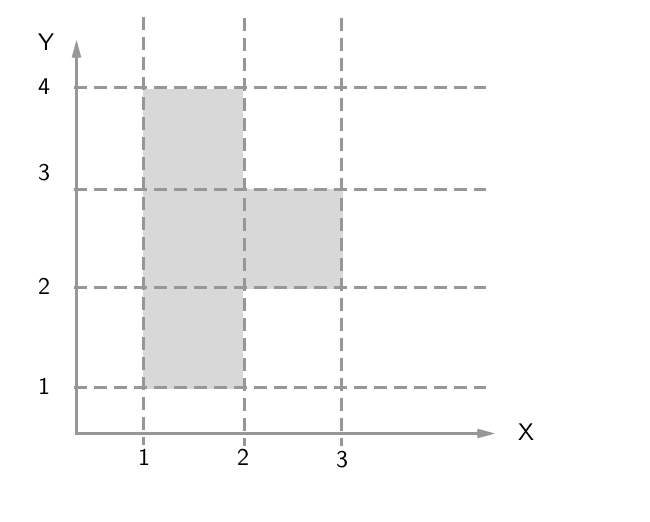
\includegraphics[height=5cm]{prob2-fig}

                The area of this shape is $4$, so $c = \frac{1}{4}$. $X$ and $Y$ are not independent, notice that if $X = 0.5$, then $Y$ can take any value between 1 and 4, but if $X = 2.5$, $Y$ can only take
                values between 2 and 3! So the distribution of $Y$ changes depending on which `slice' of $X$ we're looking at, which means they cannot be independent.

                In general, no independent variables can have a support whose shape is like the picture above. Independent variables always have a support that is rectangular.
            \end{solution}
            \item Find the marginal distributions of $X$ and $Y$.
            \begin{solution}
                You can do this with the formula $f_X(x) = \int_{-\infty}^{\infty} f_{X, Y}(x, y) dy$, and the equivalent one for $Y$. Just notice the `region of support', or where $f_{X, Y}(x, y) > 0$, changes depending on the value of $x$ or $y$ you're conditioning
                on.
                
                More intuitively, notice that the formula for $f_X(x)$ really just measures the `length' of the slice because this is a uniform distribution. For $x = 0.5$, this length is 3, and for $x = 2.5$, this length is 1. Then we might try to write: \[
                    f_X(x) = \begin{cases}
                        3 & \text{if } 1 < x < 2 \\
                        1 & \text{if } 2 < x < 3 \\
                        0 & \text{otherwise}
                    \end{cases}
                \]
                This represents the relative heights correctly, but $\int_{-\infty}^{\infty} f_X(x) dx \neq 1$! If we divide by $4$, this gives us a valid distribution: \[
                    f_X(x) = \begin{cases}
                        \frac{3}{4} & \text{if } 1 < x < 2 \\
                        \frac{1}{4} & \text{if } 2 < x < 3 \\
                        0 & \text{otherwise}
                    \end{cases}
                \]
                It's a very similar process to find the distribution for $Y$: \[
                    f_Y(y) = \begin{cases}
                        \frac{1}{2} & \text{if } 2 < y < 3 \\
                        \frac{1}{4} & \text{if } y \in [1, 2] \cup [3, 4] \\
                        0 & \text{otherwise}
                    \end{cases}
                \]
            \end{solution}
        \end{enumerate}
        \item (Spring 2017, 7.1) Consider a point $(x, y)$ is chosen uniformly from the area below:

        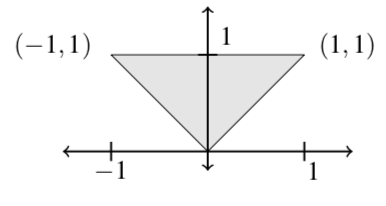
\includegraphics[height=3cm]{prob-dist.png}

        Are $X$ and $Y$ independent? What is $Pr(Y > X)$? $E[X]$? $E[Y]$?
        \begin{solution}
            They are not independent for the same reason that they weren't in problem 2, the distribution of $X$ changes conditioning on $Y$. $Pr(Y > X) = 1$, because notice that the triangle sits above the graph of $y = x$, which defines all points $(x, y)$ where $y > x$.

            $E[X] = 0$ by symmetry, the triangle is equally spread across both sides of the $y$ axis.

            To find $E[Y]$, we need to calculate the marginal distribution of $Y$. It's easier to calculate $P(Y \leq y)$, the CDF (this is an extremely common trick! if you can't figure out the pdf, try the cdf first). Imagine a horizontal line at $Y = y$.
            The probability that $Y \leq y$ is the area of that triangle divided by the area of the entire triangle (which is 1). The triangle lying under the horizontal line $Y = y$ has height $y$ and base $2y$, so has area $y^2$. Then \[
                P(Y \leq y) = y^2
            \]
            So $f_Y(y) = 2y$, so to find $E[Y]$: \[
                E[Y] = \int_{0}^1 y \cdot 2 y^2 dy = \left[\frac{2}{3} y^3 \right]_{0}^1 = \frac{2}{3}
            \]
        \end{solution}
        \item (Fall 2017, 6.4) Let $X_1, \ldots X_n$ be i.i.d $U[0, 1]$ random variables.
        \begin{enumerate}
            \item Find the PDF of $Y = \text{min}(X_1, \ldots, X_n)$.
            \begin{solution}
                Once again, it's easier to find the CDF. $P(Y \leq y) = P(X_1 \leq y \cup \ldots \cup X_n \leq y) = 1 - P(X_1 > y \cap \ldots \cap X_n > y) = 1 - P(X_1 > y) \cdot \ldots \cdot P(X_n > y)$. As $P(X_n > y) = 1 - y$, we have \[
                    P(Y \leq y) = 1 - (1 - y)^n
                \]

                We used the trick that sometimes it is easier to find $P(Y \geq y)$ instead of $P(Y \leq y)$. Keep your eye out, but the first one is often better for $min$ problems and the second one is better for $max$ problems.

                Now to find the PDF, we take the derivative: \[
                    f_Y(y) = n(1 - y)^{n-1}
                \]
            \end{solution}
            \item Let $Z = \text{max}(X_1, \ldots, X_{100})$. What is $E[Z]$?
            \begin{solution}
                One way to do this is as we did before. Then the the CDF of $Z$ is \[
                    P(Z \leq z) = (1 - z)^{100}
                \] so the PDF is $f_Z(z) = 100(1 - z)^{99}$. So we can find the expectation with the not-too-terrible integral: \[
                    \int_{0}^1 z \cdot 100 (1-z)^{99} dz = \frac{100}{101}\left[z^{101}\right]_0^1 = \frac{100}{101}
                \]

                Another way to do this is to notice that $X_1, \ldots X_{100}$ divide $[0, 1]$ into $101$ `compartments'. By symmetry we expect all these compartments to be the same size, and $E[Z]$ is just one minus the size of the rightmost compartment, which is $1 - \frac{1}{101} = \frac{100}{101}$.
            \end{solution}
        \end{enumerate}
        \item (Fall 2017, 6.13) Let $X \sim \text{Exp}(\lambda)$, and let $\lceil X \rceil$ denote the ceiling of $X$ (the smallest integer greater than or equal to $X$). Find the distribution of $\lceil X \rceil$.
        Does it look like a distribution we've seen before? What parameters?
        \begin{solution}
            We talked last time about how the geometric is the discrete analog of the exponential distribution. So let's \textit{guess} that $\lceil X \rceil$ has the distribution: \[
                P(\lceil X \rceil = k) = (1 - p)^{k-1} p
            \]
            What's left is to find $p$. By how the ceiling is defined, all the values $x$ for which $\lceil x \rceil = 2$, for instance, lie between $1$ and $2$. So in general, \[
                P(\lceil X \rceil = k) = P(k - 1 < X < k) = \int_{k-1}^{k} \lambda e^{-\lambda x} dx
            \]
            Another way to evaluate this is to notice $P(k - 1 < X < k) = P(X < k) - P(X < k - 1)$ and use the CDF for the Exponential distribution: \[
                P(X < k) - P(X < k - 1) = (1 - e^{-\lambda k}) - (1 - e^{-\lambda (k - 1)})
            \] \[
                = e^{- \lambda (k - 1)} - e^{- \lambda k} = e^{-\lambda (k - 1)}(1 - e^{-\lambda}) = \left(e^{-\lambda}\right)^{k-1}(1 - e^{- \lambda})
            \]
            This looks exactly like a geometric with $p = e^{-\lambda}$, wow!

            I will be the first to admit that these simple 5 equalities could actually be really hard to do in a final environment (I certainly choked trying to do it in class). There, it's always a good idea
            to follow your nose and intuition, make guesses! If it takes you too long, give some semi-reasonable answer and move on to another problem. It's almost certainly worth it to move on than wrestle with algebra,
            and CS 70 is definitely not a class about wrestling with algebra anyways.
        \end{solution}
        \item (Fall 2017, 6.14) Let $X \sim N(0, 1)$ and $Y \sim N(1, 1)$ be independent Gaussian random variables. You get an observation $z = 0.6$ that is equally likely to come from $X$ and $Y$. You want to decide whether $z$ came from $X$ or $Y$ by evaluating which decision
        leads to a larger probability of being right.
        \begin{enumerate}
            \item If you decide $z$ came from $X$, what is the probability you are right?
            \begin{solution}
                We need the pdf of the normal distribution: \[
                    f_X(x) = \frac{1}{\sqrt{2 \pi \sigma^2}} e^{\frac{-(x - \mu)^2}{2 \sigma^2}}
                \]
                What a scary formula. All we're going to do is plug some values into it, so everything is going to be okay. There's no easy way to find the CDF, so if you ever need to leave things in terms of the CDF, write $\Phi(x)$, defined as: \[
                    \Phi(x) = \int_{\infty}^x \frac{1}{\sqrt{2 \pi \sigma^2}} e^{\frac{-(x - \mu)^2}{2 \sigma^2}} dx
                \] (although the exam will probably tell you when to leave things
                in that form).

                This question is phrased weirdly. We are flipping a coin to decide between $X$ and $Y$, and then sampling from whichever distribution we picked. The value we sampled is $z = 0.6$, and so long as the pdf is different at $0.6$ between $X$ and $Y$, that means
                that actually tells us information about which distribution it came from. We use the law of total probability: \[
                    P(\text{coin picked } X \mid z = 0.6) = \frac{P(\text{coin picked } X \cap z = 0.6)}{P(\text{coin picked } X \cap z = 0.6) + P(\text{coin picked } Y \cap z = 0.6)}
                \]
                Each of these events are now just evaluating the normal distribution PDF! All have a factor of $\frac{1}{\sqrt{2 pi}}$, so I exclude that to stay sane. So we get \[
                    P(\text{coin picked } X \mid z = 0.6) = \frac{e^{-0.6^2/2}}{e^{-0.6^2/2} + e^{-0.4^2/2}}
                \]
            \end{solution}
            \item Should you decide $z$ is from $X$ or from $Y$ to get a larger probability of being right?
            \begin{solution}
                We're thinking in a very Bayesian way here. If we had no information about the sample, the probability the coin flip picked $X$ or $Y$ is exactly 1/2. But knowing the sample gives us some information about which one. Because \[
                    P(\text{coin picked } X \mid z = 0.6) = 1 - P(\text{coin picked } Y \mid z = 0.6)
                \]
                we should only guess $X$ if $P(\text{coin picked } X \mid z = 0.6) > 0.5$. But $e^{-0.6^2/2} < e^{-0.4^2/2}$, meaning that this probability is less than $0.5$, so we should guess $Y$ instead.
            \end{solution}
        \end{enumerate}
        \item (Spring 2017, 7.2) You pick a real number from the range [0, 1] using the uniform distribution. Then your friend independently picks a real number uniformly at random from the range [0, 2].
        \begin{enumerate}
            \item What is the probability that your two numbers differ by no more than one?
            \begin{solution}
                We did not talk about this, so will not give solution away here. You can check on TBP or hkn to see exam solutions.
            \end{solution}
            \item Now you pick a variable in the range [0, 1] with pdf $f(x) = 2x$. Then your friend still picks a real number uniformly at random from [0, 2]. Now what is the probability that your two numbers differ by no more than one?
            \begin{solution}
                We did not talk about this, so will not give solution away here. You can check on TBP or hkn to see exam solutions.
            \end{solution}
        \end{enumerate}
     \end{enumerate}
    \end{document}
        